\begin{frame}
    \frametitle{Ende-zu-Ende-Verschlüsselung}
    \begin{center}
      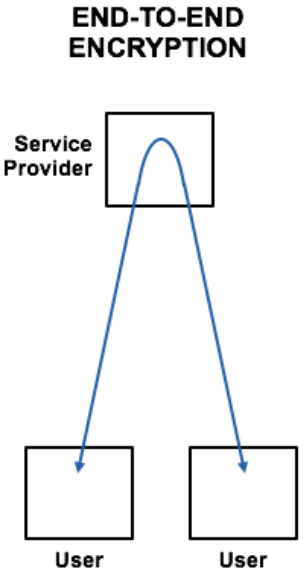
\includegraphics[height=0.8\textheight]{img/enc-e2e.png}
    \end{center}
\end{frame}

\note{Ende-zu-Ende-Verschlüsselung ist die einzige wirklich wirksame, weil sie nicht nur Angreifer im offenen Internet ausschließt sondern auch den Dienstbetreiber selbst. Diesem muss man jedoch oft trotzdem ein gewisses Vertrauen entgegenbringen, weil der Betreiber in vielen Fällen die Software ausliefert oder die Leute miteinandern in Verbindung bringt. Eine sinnvolle Nutzung ist nur gewährleistet, wenn die Software Open Source ist und die Nutzer sich gegenseitig ``bestätigen'' können --- meist über eine Sicherheitsfrage oder einen scannbaren Barcode.}

\begin{frame}
  \frametitle{Identität}
    \begin{center}
      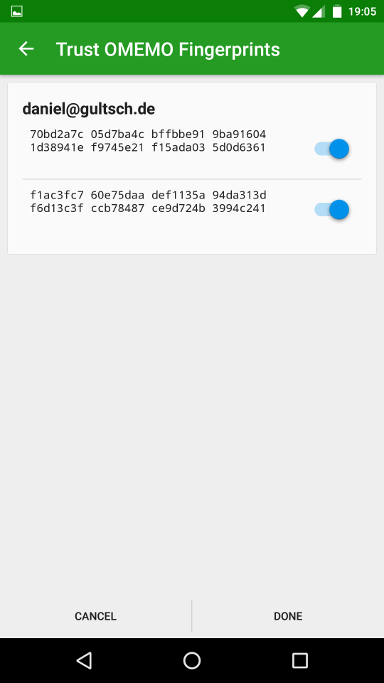
\includegraphics[height=6cm]{img/conversations-identity.jpg}
      \vspace{2cm}
      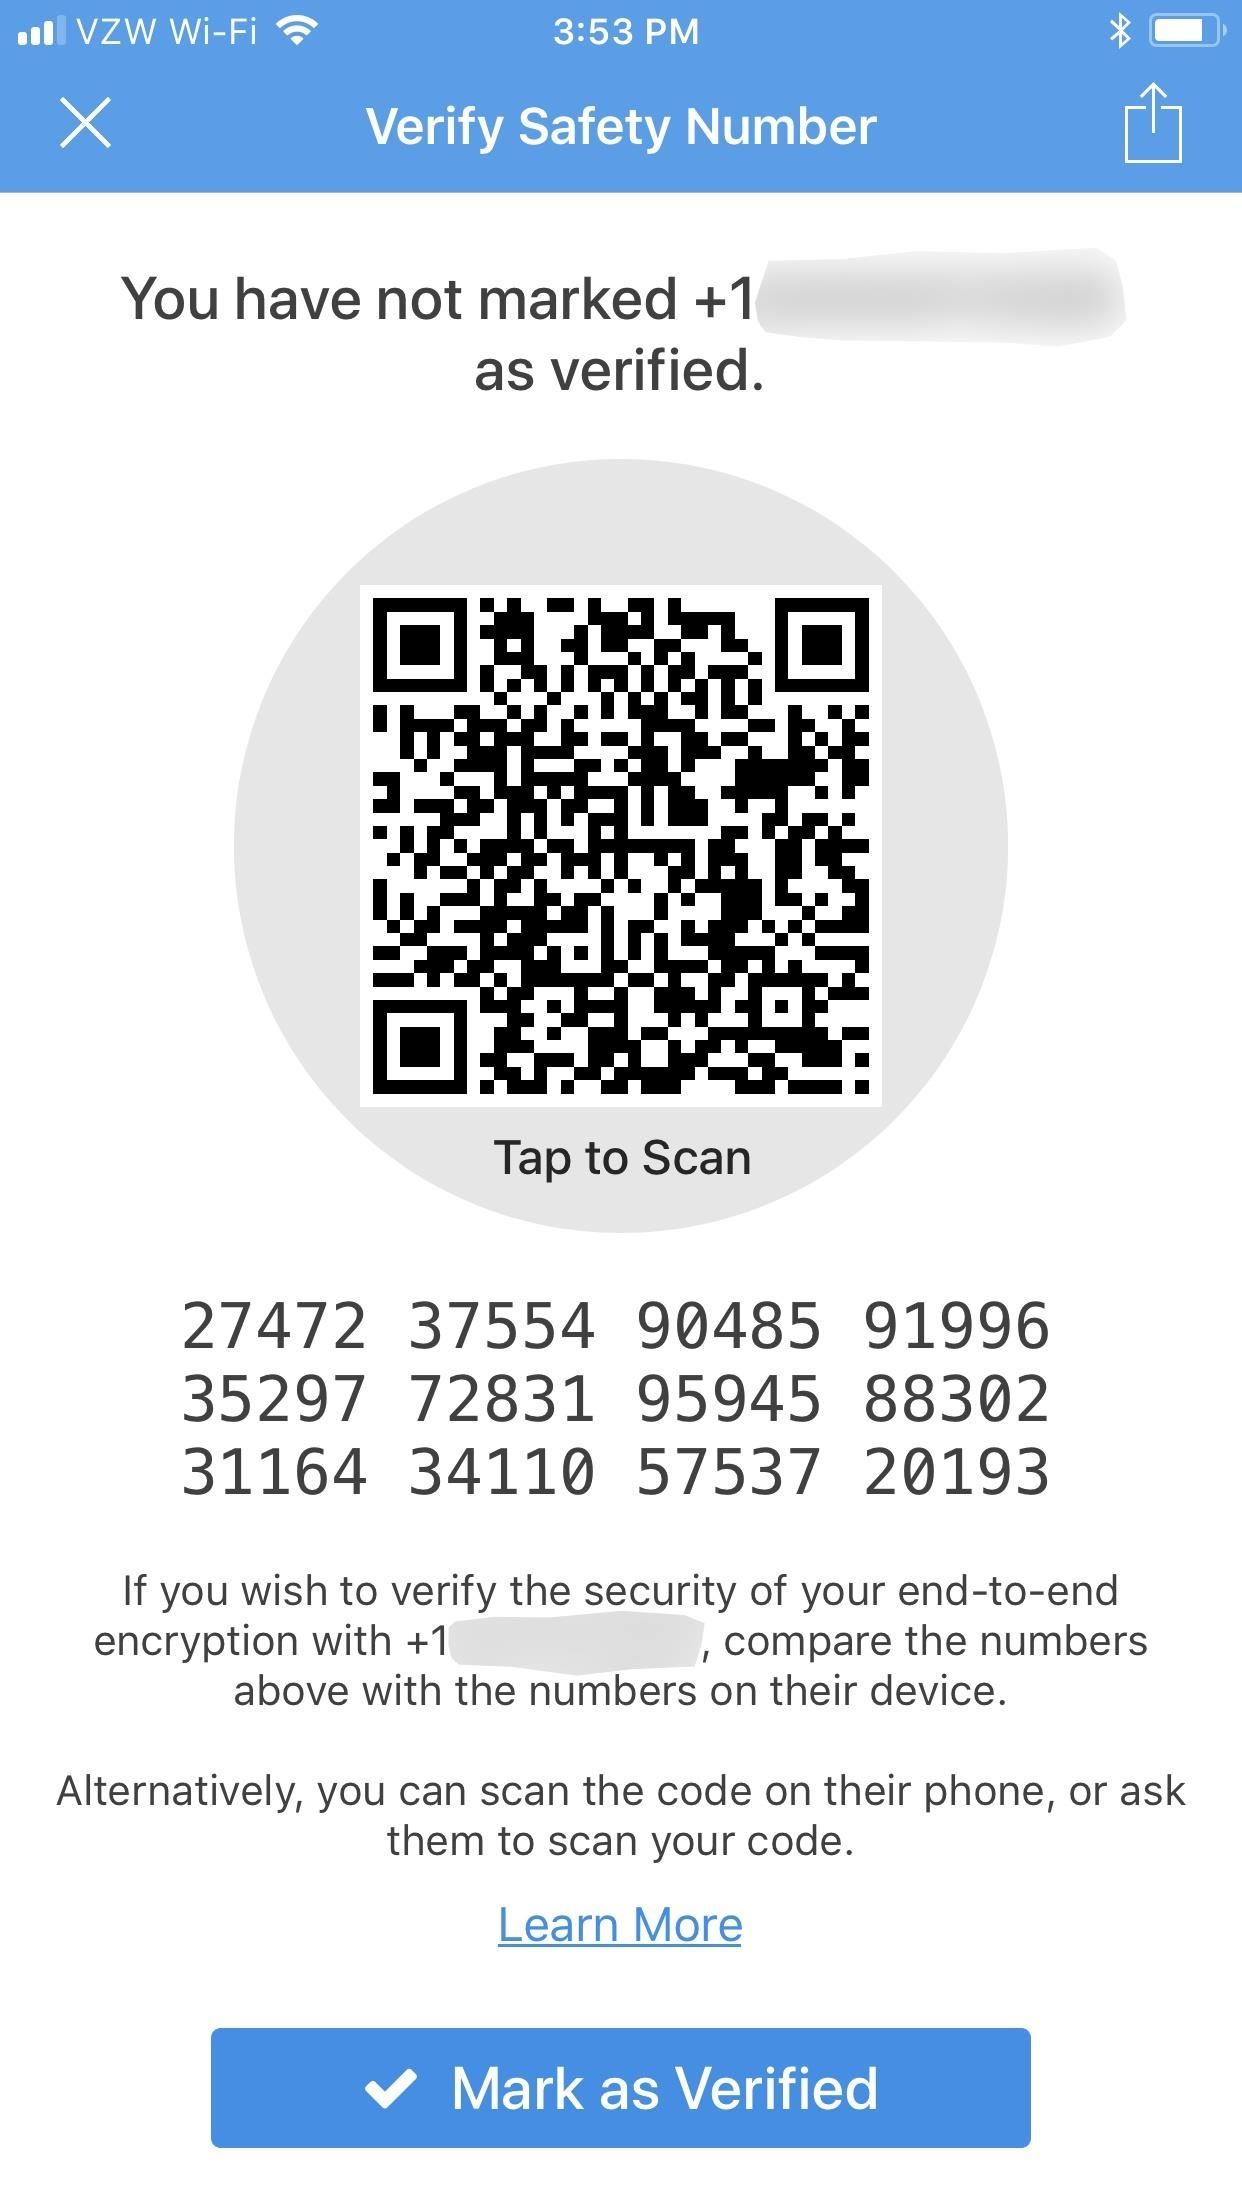
\includegraphics[height=6cm]{img/signal-identity.jpg}
    \end{center}
\end{frame}

\begin{frame}
  \frametitle{PGP (Pretty Good Privacy)}
  \begin{center}
    
\includegraphics[height=0.1\textheight]{img/gpg.png}
  \end{center}
  \begin{itemize}
    \item<2->Hauptsächlich für Emailverschlüsselung genutzt
    \item<3->Integration in Thunderbird (Enigmail), Outlook (Gpg4win), online mail (Mailvelope)
    \item<4->Vorteile: Gilt seit Jahr(zehnt)en als sicher, 
    \item<5->Schwer benutzbar, keine ``Forward Secrecy''
  \end{itemize}
\end{frame}

\note{PGP ist die bekannteste Möglichkeit für E2E-Verschlüsselung von Emails. Das dafür notwendige Programm GnuPG bzw. GPG ist ist Open Source, man kann sich gegenseitig Bestätigen und es gibt Plugins für Thunderbird und Outlook. Sogar Webmail (z.B. Gmail) kann man damit absichern, wenn man das Browseraddon Mailvelope benutzt. Web.de und GMX haben dafür sogar eine einfache Einrichtungsmöglichkeit auf der Website geschaffen, aber es funktioniert auch sonst überall. GPG ist jedoch trotzdem nicht für einfache Benutzung bekannt, der Link erklärt wie man es einrichtet.}

\begin{frame}
  \frametitle{PGP:\@ Email-Verschlüsselung}
  \begin{center}
    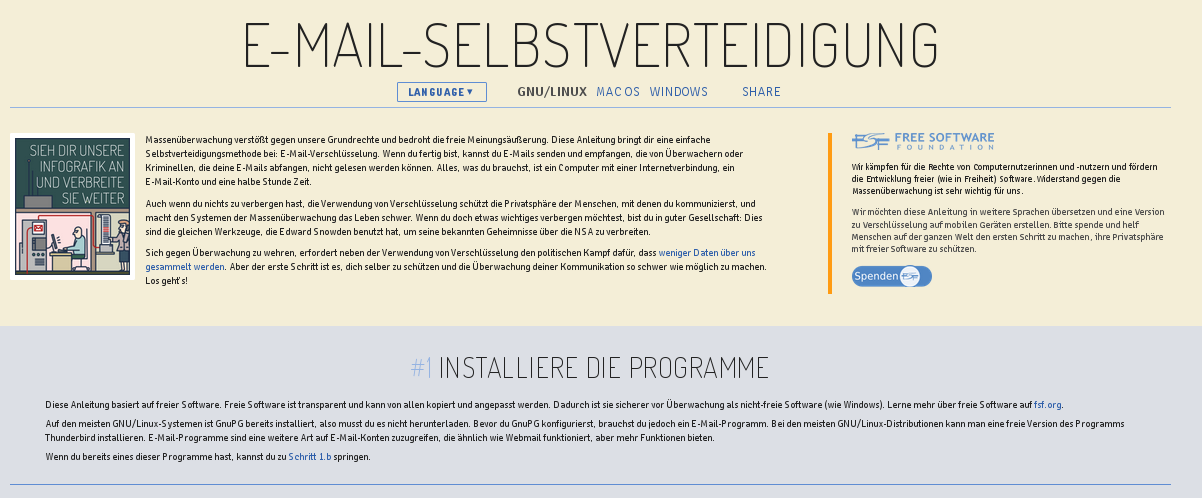
\includegraphics[height=0.5\textheight]{img/emailselfdefense.png}
    \begin{itemize}
      \item https://emailselfdefense.fsf.org/de/
    \end{itemize}
  \end{center}
\end{frame}

\begin{frame}
  \frametitle{OTR (Off the Record)}
  \begin{itemize}
    \item<2->Genutzt für Chat/Messaging (z.B. in Jabber/XMPP)
    \item<3->Vorteile: Forward Secrecy
    \item<4->Nachteile: Kein Multi-Device, keine Offlinenachrichten
  \end{itemize}
\end{frame}

\begin{frame}
  \frametitle{Signalprotokoll}
  \begin{center}
    
\includegraphics[height=0.2\textheight]{img/signal-logo.png}
  \end{center}
  \begin{itemize}
    \item<2->Eingeführt vom Signal Messenger
    \item<3->Mittlerweile auch von Whatsapp und anderen Messengern benutzt
    \item<4->Bei Jabber als OMEMO bekannt
    \item<5->Vorteile: Forward Secrecy, Multi-Device, Offlinenachrichten
  \end{itemize}
\end{frame}

\begin{frame}
  \frametitle{Jabber: Conversations, ChatSecure}
    \begin{center}
      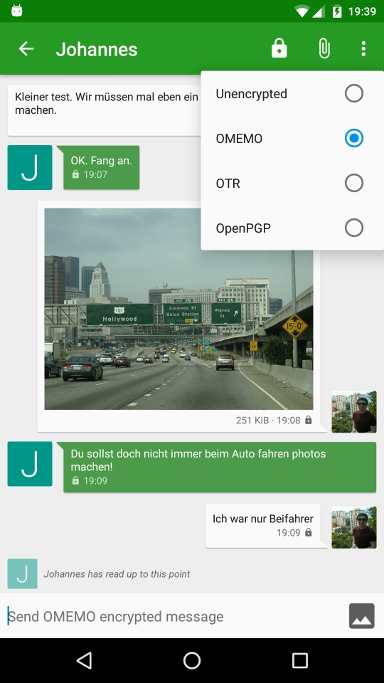
\includegraphics[height=6cm]{img/conversations.jpg}
      \hspace{0.5cm}
      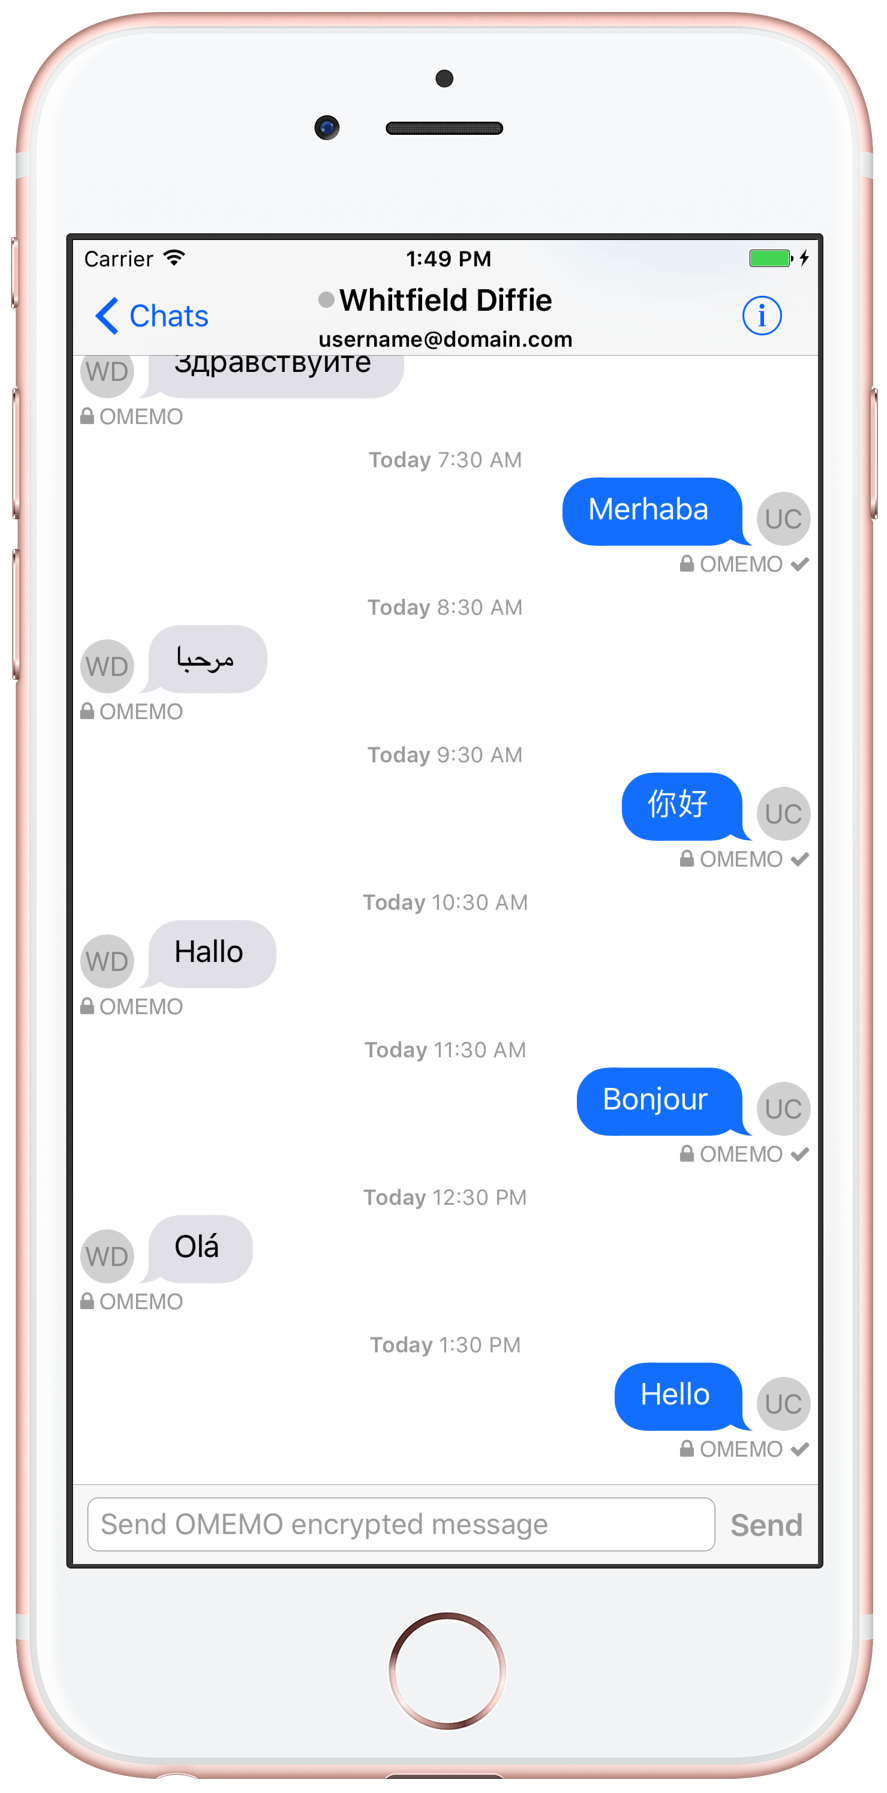
\includegraphics[height=6cm]{img/chatsecure.png}
    \end{center}
    \url{https://xmpp.net/directory.php}
\end{frame}

\note{Einfacher ist die Nutzung von E2E-Verschlüsselung bei diversen Messengern. Jabber, auch XMPP genannt, ist eine gute Option, weil es ein offenes Protokoll wie Email ist. Man kann sich seinen Anbieter selbst aussuchen und hat dann einen Nutzernamen, der so wie eine Emailadresse aussieht, z.B. thomas@jabber.de. Eine Liste mit Jabberservern und ihre Qualität ist unter dem Link zu finden.}

\begin{frame}
  \frametitle{Signal}
    \begin{center}
      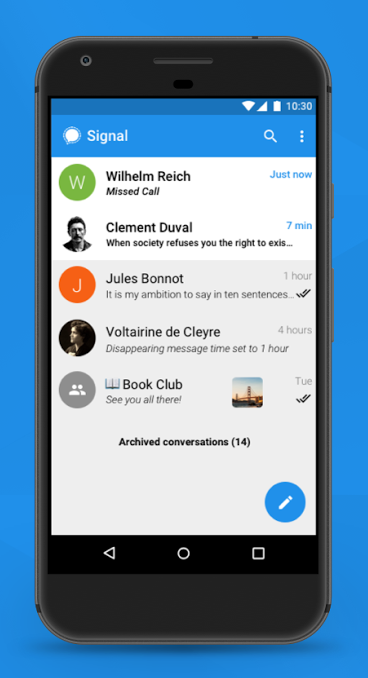
\includegraphics[height=6cm]{img/signal-android.png}
      \hspace{0.5cm}
      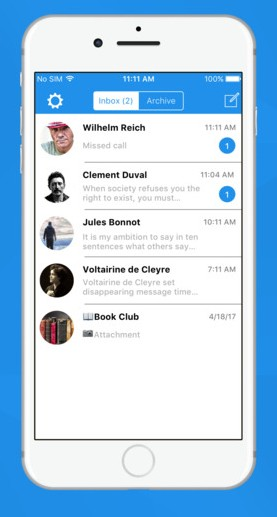
\includegraphics[height=6cm]{img/signal-ios.jpg}
    \end{center}
\end{frame}

\note{Noch einfacher nutzbar ist Signal, ein Open Source und E2E-verschlüsselter Messenger, der von einer gemeinnützigen Organisation betrieben wird und sogar von Edward Snowden selbst empfohlen wird. Es funktioniert sehr ähnlich wie Whatsapp und kann auch Bilder und Videos verschicken. Ein Nachteil ist jedoch, dass es trotzdem ein zentraler Dienst ist und man sich nicht wie bei Jabber oder Email seinen Anbieter und damit auch den Ort an dem die Daten (z.B. die Freundesliste) liegen aussuchen kann.}
